% ideias:
% etimologia prosodia
% rant bret victor

\documentclass{beamer}

\usepackage[utf8]{inputenc}     % Encoding certo
\usepackage[brazilian]{babel}   % Hifenização e dicionário

\usepackage{amsmath}
\usepackage{amsfonts}
\usepackage{amssymb}

\setbeamertemplate{navigation symbols}{}  % Esconde o menu tosco
\usetheme{Madrid}
\useinnertheme{rectangles}
\usefonttheme{professionalfonts}
% \usefonttheme{serif}            % A versão sem serifa é horrível
\usepackage{times}

\setbeamertemplate{blocks}[default]

\title[Geração de prosódia]{Geração de prosódia para o português brasileiro em sistemas text-to-speech}

\author{Felipe Cortez de Sá}
\date{Junho de 2018}
\institute[UFRN]{Universidade Federal do Rio Grande do Norte}

\begin{document}

\begin{frame}
  \titlepage
\end{frame}

\begin{frame}{Resumo}
  \tableofcontents
\end{frame}

\section{Introdução}
\begin{frame}{Motivação}
  \begin{itemize}
    \item \emph{Voice User Interfaces}
        \begin{itemize}
            \item \emph{Apple - Siri}
            \item \emph{Google Assistant}
            \item \emph{Microsoft - Cortana}
            \item \emph{Amazon - Alexa}
        \end{itemize}
    \item Acessibilidade
  \end{itemize}
\end{frame}

\section{Prosódia}
\begin{frame}{Prosódia}
  \begin{itemize}
    \item O que é prosódia?
        \begin{itemize}
            \item pros, "verso"
            \item odé,  "canto"
        \end{itemize}
  \end{itemize}
  \pause
    \begin{figure}
      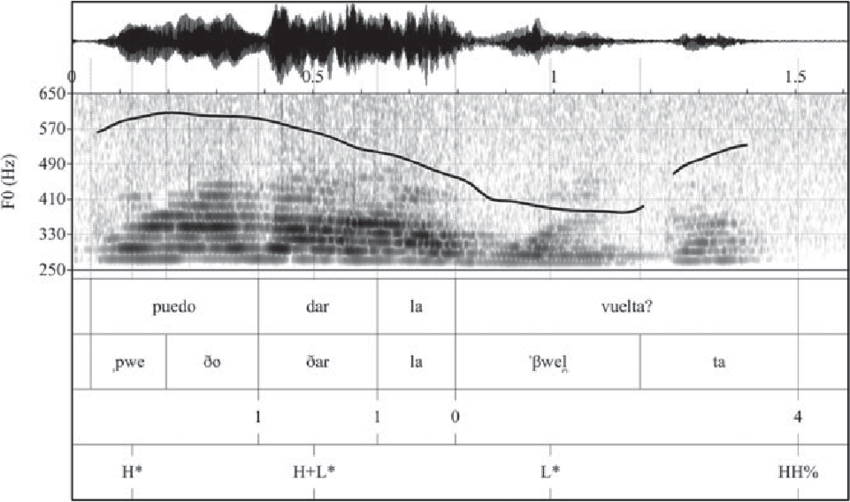
\includegraphics[scale=0.25]{prosody.png}
    \end{figure}
\end{frame}

\begin{frame}{Prosódia}
  \begin{itemize}
    \item Afetiva (pura)
    \item Suprasegmental
    \item Aumentativa
  \end{itemize}
\end{frame}

\section{TTS}
\begin{frame}{Sistemas TTS}
  \begin{block}{Arquitetura genérica}
    \begin{figure}
      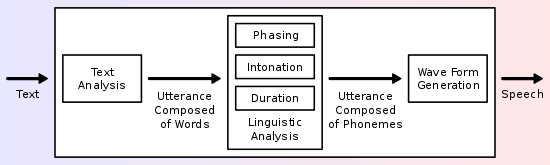
\includegraphics[scale=0.55]{tts-system.png}
    \end{figure}
  \end{block}
\end{frame}

\begin{frame}{Prosódia em sistemas TTS}
  \begin{itemize}
    \item Prosódia neutra
    \item Prosódia aprendida
    \item SSML -- \emph{Speech Synthesis Markup Language}
  \end{itemize}
\end{frame}

\begin{frame}{Sistemas TTS}
  \begin{itemize}
    \item Comerciais
      \begin{itemize}
        \item CereProc
        \item Ivona (Amazon)
        \item Watson (IBM)
      \end{itemize}
    \item Open-source
      \begin{itemize}
        \item MaryTTS
        \item espeak-ng
        \item Merlin
      \end{itemize}
  \end{itemize}
\end{frame}

\begin{frame}{Abordagens}
  \begin{itemize}
    \item Dífonos (MBROLA)
    \item Unit selection (MaryTTS)
    \item Síntese paramétrica (espeak-ng)
    \item DNN (Merlin)
  \end{itemize}
\end{frame}

\section{Implementação}
\begin{frame}{Teoria}
  \begin{itemize}
  \item ToBI (Tone Breaks and Indices)
    \begin{itemize}
    \item Usado por análises feitas por Moraes para pt-br
    \item Usado pelo grupo de pesquisas de TTS da CMU / UoE
    \item Pierrehumbert (modelo \emph{Autosegmental-Metrical})
    \end{itemize}
  \item INTSINT
  \item IPO
  \end{itemize}
\end{frame}

\begin{frame}{Ferramentas}
  \begin{itemize}
    \item Python 3
    \item espeak-ng (front-end)
    \item MBROLA (back-end)
    \item Módulo gráfico
  \end{itemize}
\end{frame}

\begin{frame}{Trabalhos futuros}
  \begin{itemize}
    \item Usar \emph{Natural Language Understanding} para adivinhar prosódia
    \item Gerar prosódia a partir de marcação SSML
  \end{itemize}
\end{frame}
\end{document}
